\documentclass{article}
\usepackage{pgfplots}
\pgfplotsset{compat=1.16}

\begin{document}

\begin{figure}[h]
    \centering
    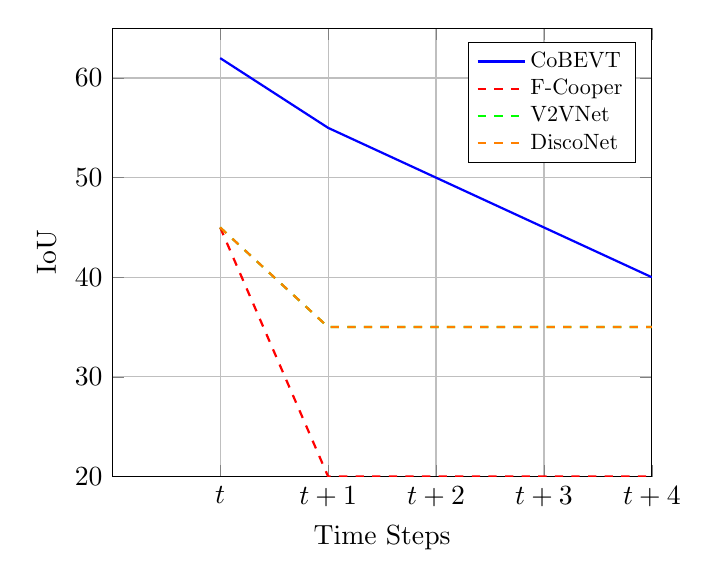
\begin{tikzpicture}
        \begin{axis}[
            xlabel={Time Steps},
            ylabel={IoU},
            legend pos=north east,
            legend cell align=left,
            legend style={nodes={scale=0.8, transform shape}},
            xmin=0, xmax=5,
            ymin=20, ymax=65,
            xtick={1,2,3,4,5},
            xticklabels={$t$, $t+1$, $t+2$, $t+3$, $t+4$},
            ytick={20, 30, 40, 50, 60},
            yticklabels={20, 30, 40, 50, 60},
            grid=major,
            ]
            
            \addplot[blue, thick, solid] coordinates {
                (1, 62)
                (2, 55)
                (3, 50)
                (4, 45)
                (5, 40)
            };
            \addlegendentry{CoBEVT}
            
            \addplot[red, thick, dashed] coordinates {
                (1, 45)
                (2, 20)
                (3, 20)
                (4, 20)
                (5, 20)
            };
            \addlegendentry{F-Cooper}
            
            \addplot[green, thick, dashed] coordinates {
                (1, 45)
                (2, 35)
                (3, 35)
                (4, 35)
                (5, 35)
            };
            \addlegendentry{V2VNet}
            
            \addplot[orange, thick, dashed] coordinates {
                (1, 45)
                (2, 35)
                (3, 35)
                (4, 35)
                (5, 35)
            };
            \addlegendentry{DiscoNet}
            
        \end{axis}
    \end{tikzpicture}
    \caption{Comparison of IoU for different models over time. Solid lines indicate the extension with TempCoBEV. Dashed lines indicate the default model. The dashed green and orange lines overlap heavily.}
    \label{fig:iou_comparison}
\end{figure}

\end{document}